\documentclass{article}
\usepackage{hyperref}
\usepackage{amsmath,amssymb}
\usepackage{graphicx}
\usepackage{caption}
\usepackage{subcaption}
\usepackage[section]{placeins}
\renewcommand{\thesubsection}{\thesection.\alph{subsection}}
\usepackage{listings}

\title{\bf{CSE397: Assignment \#2}}
\author{Nicholas Malaya \\ Institute for Computational Engineering and Sciences \\ University of Texas at Austin} \date{}

\begin{document}
\maketitle

\newpage
\section{Problem 1}

\begin{figure}[!htb]
  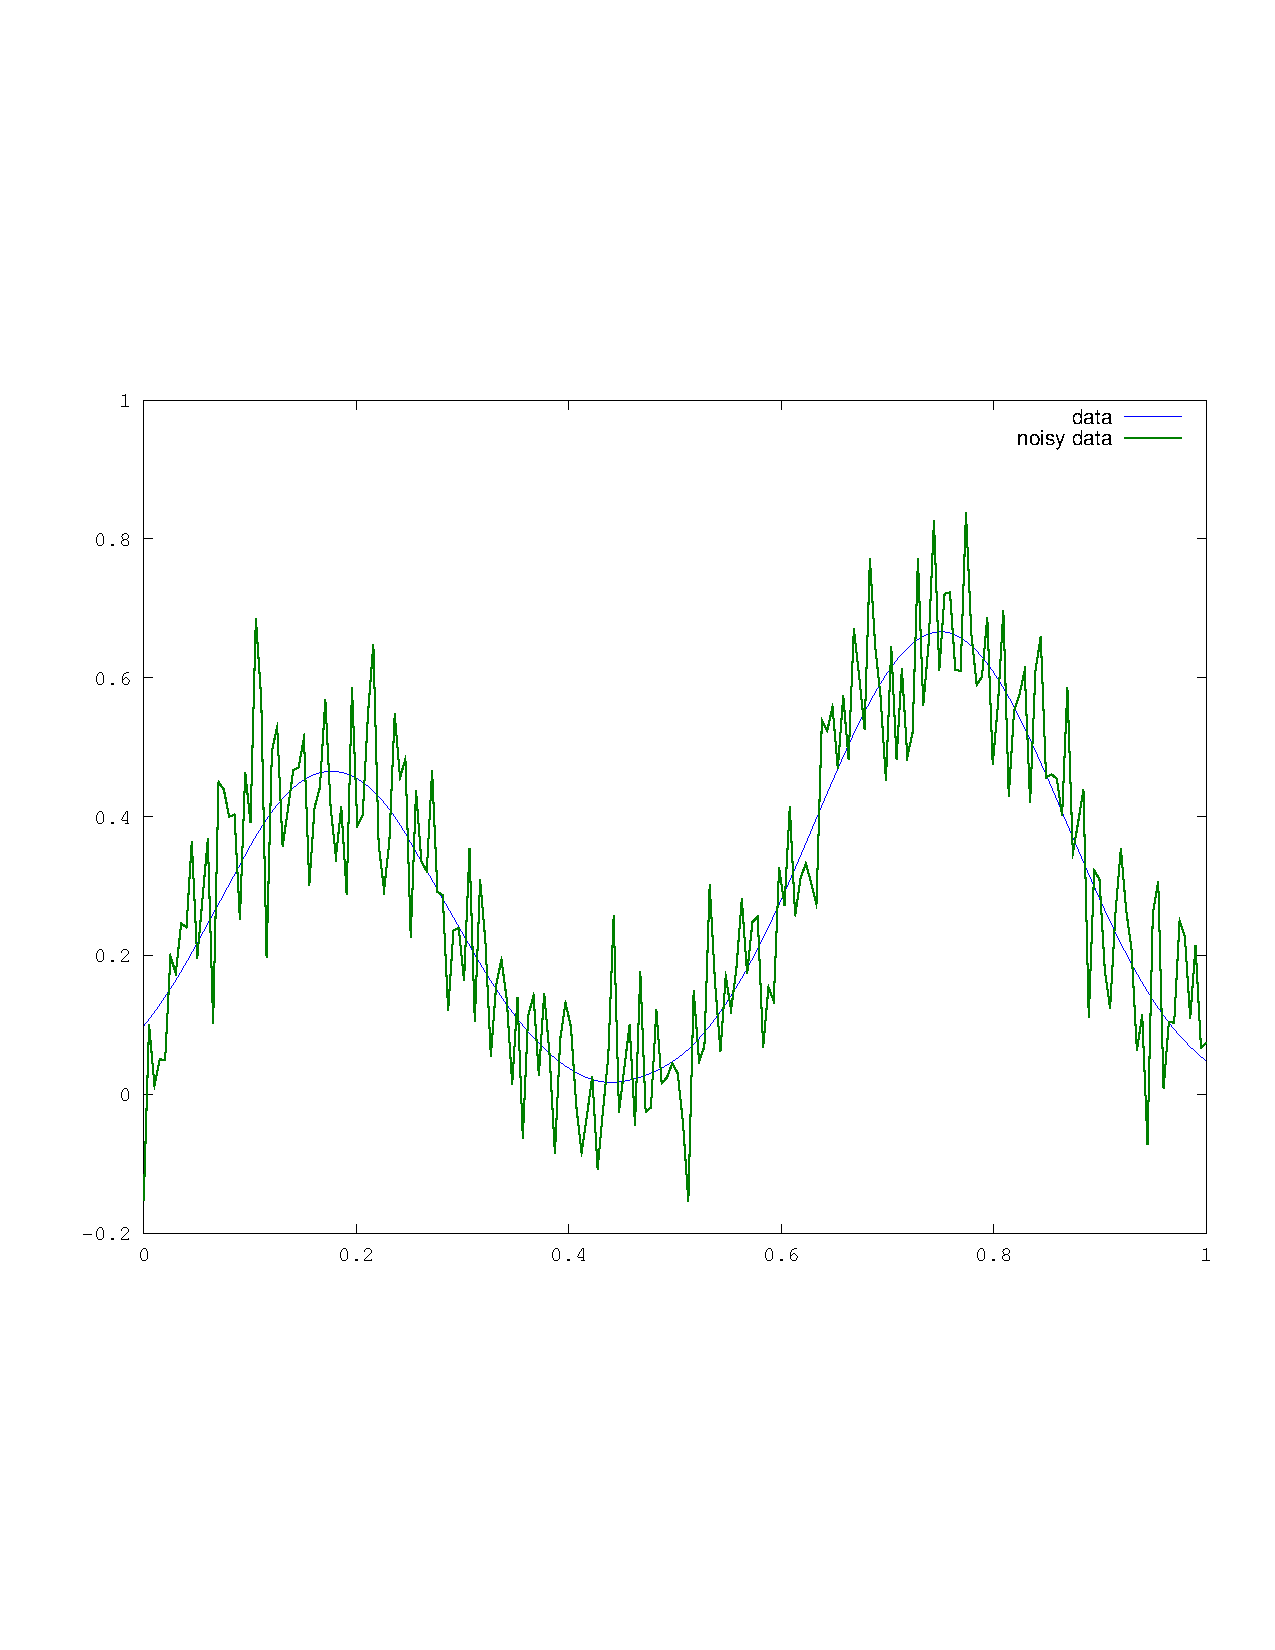
\includegraphics[scale=.5]{plots/data.pdf}
  \label{fig:data}
  \caption{The data (after applying the filter) with and without
 normally distributed noise. } 
\end{figure}

After applying the new filter $k(x)$ and adding gaussian noise, the data
used as input for the inverse problem is plotted in figure 1. 

Notice that this filter is significant: the raw data generated after
passing through the filter (even without statistical noise) has lost
several features of the underlying ``true'' signal. 

\subsection{$T_{\text{SVD}}$}


\begin{figure}[!htb]
        \centering
        \begin{subfigure}[bh]{0.45\textwidth}
                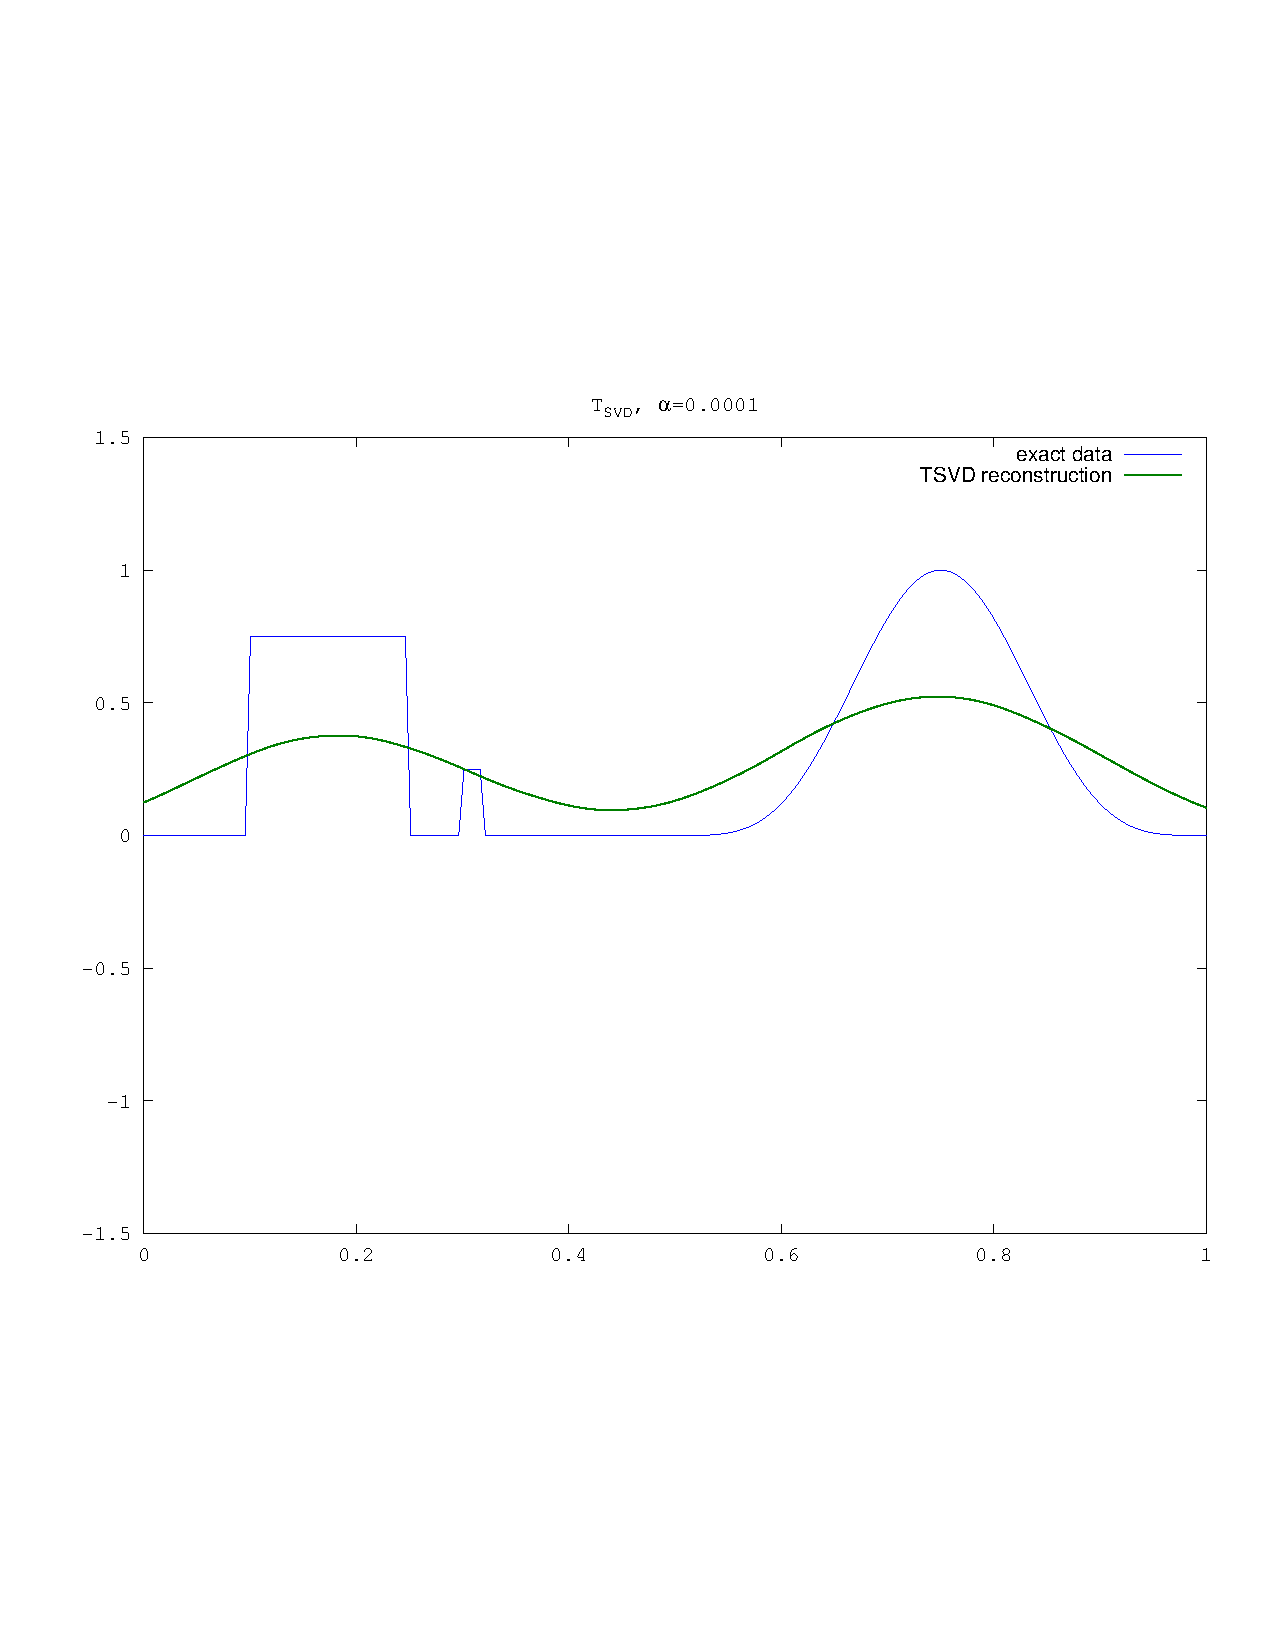
\includegraphics[width=\textwidth]{plots/tsvd0001.pdf}
                \caption{$\alpha=0.0001$}
        \end{subfigure}%
        \begin{subfigure}[bh]{0.45\textwidth}
                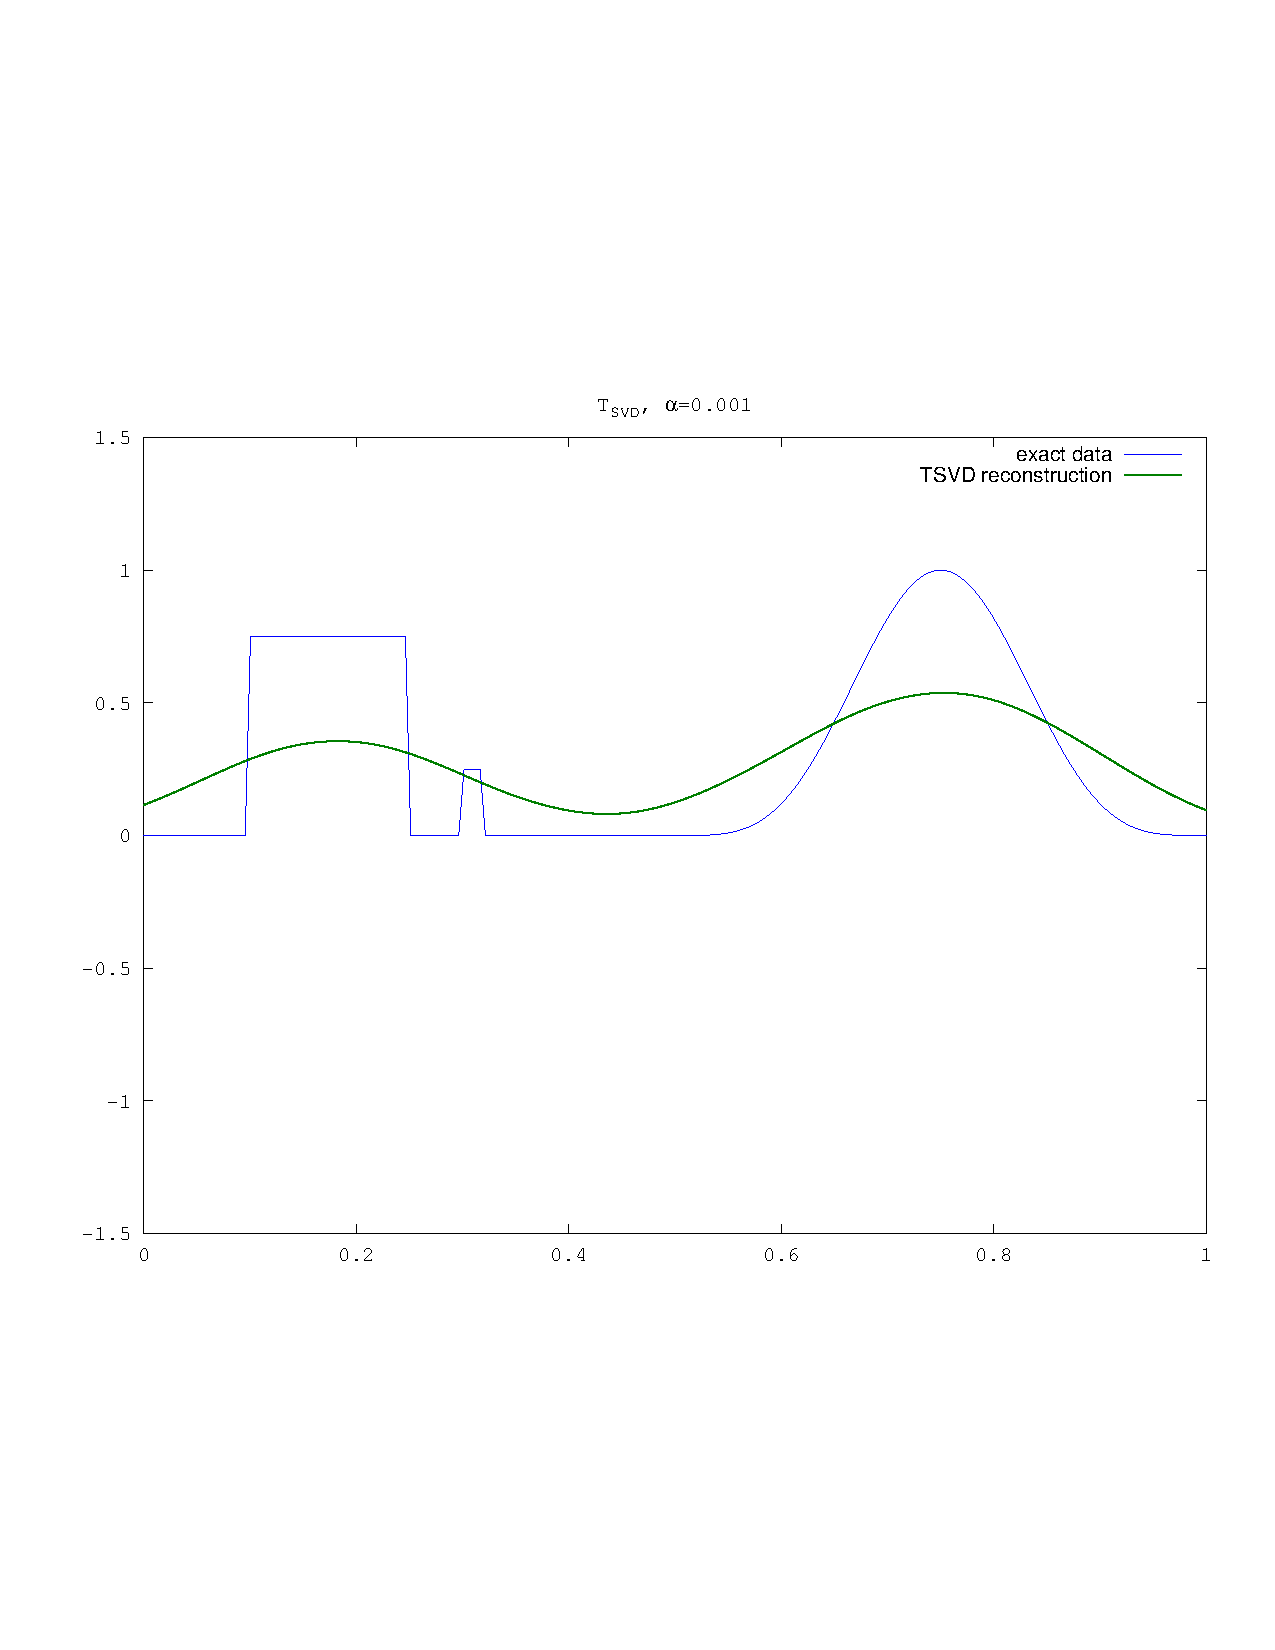
\includegraphics[width=\textwidth]{plots/tsvd001.pdf}
                \caption{$\alpha=0.001$}
        \end{subfigure}
        \centering
        \begin{subfigure}[bh]{0.45\textwidth}
                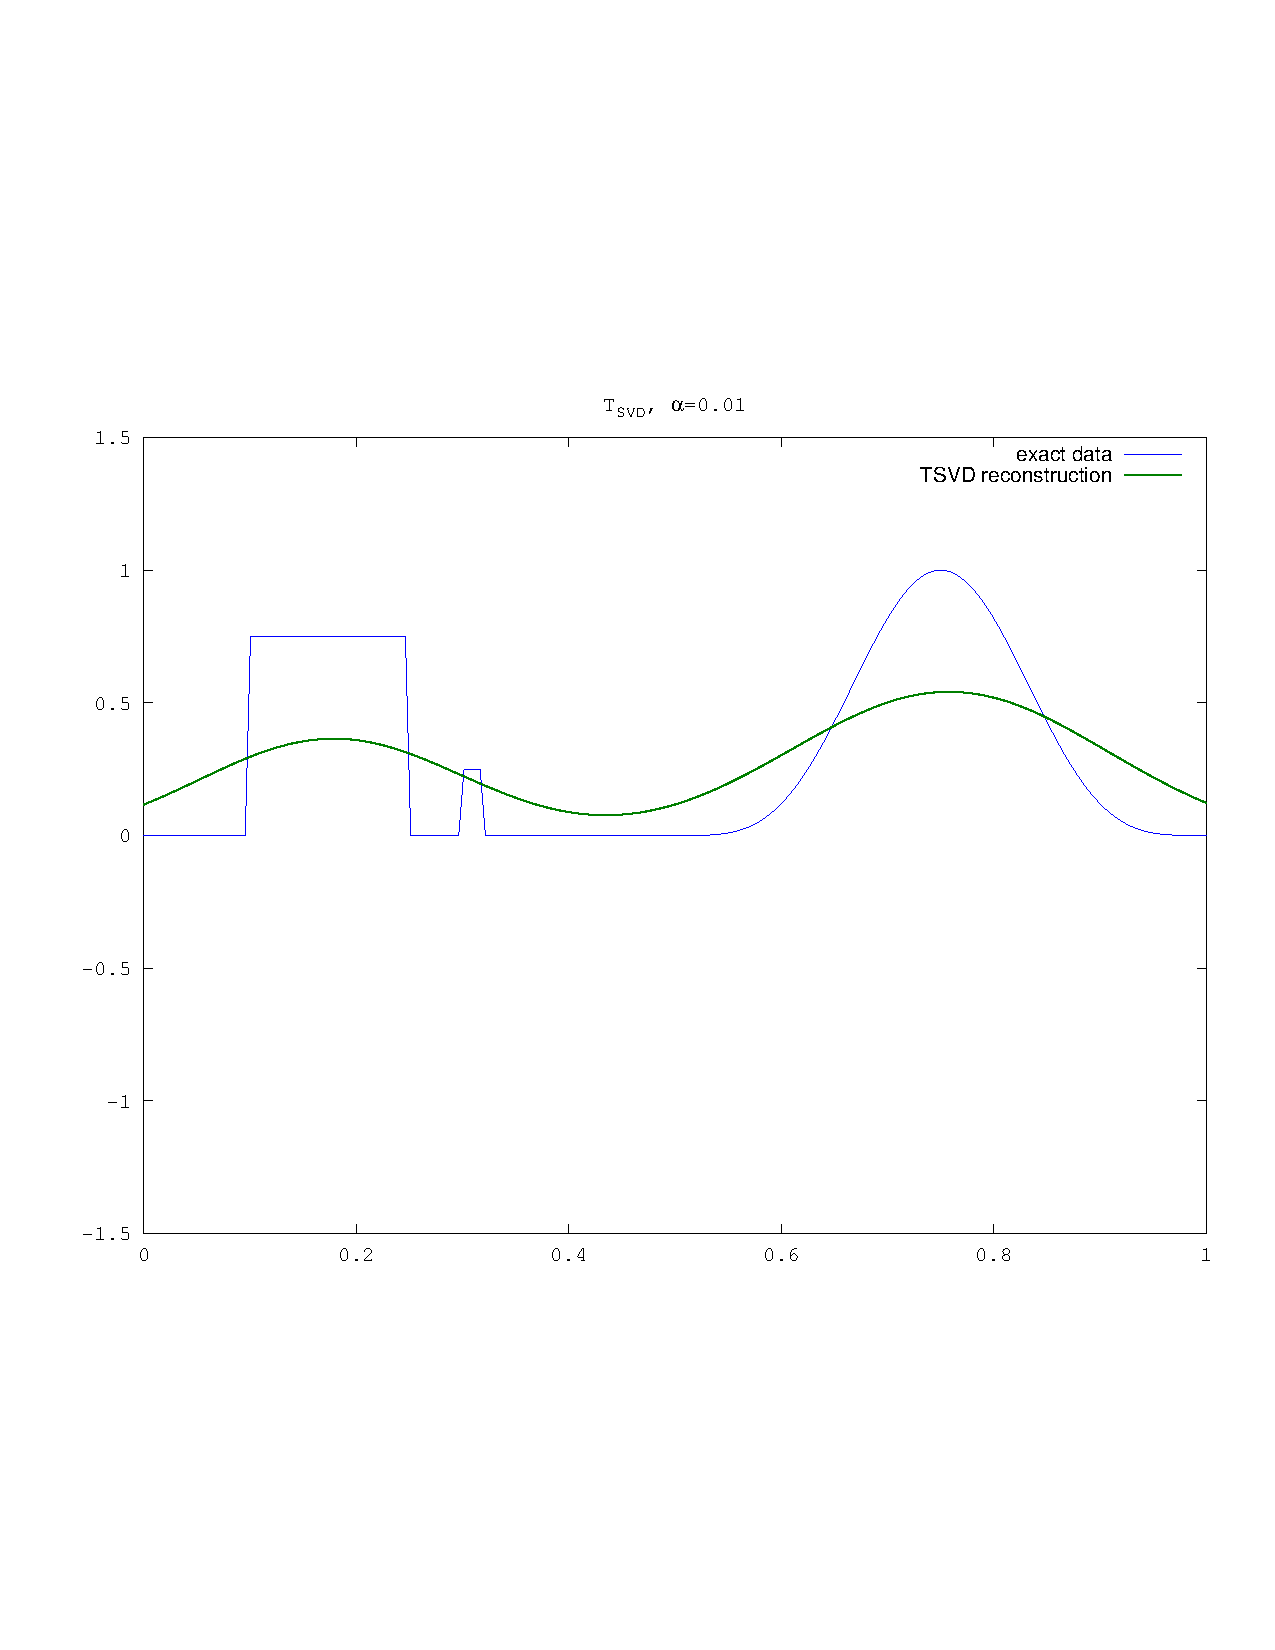
\includegraphics[width=\textwidth]{plots/tsvd01.pdf}
                \caption{$\alpha=0.1$}
        \end{subfigure}%
        \begin{subfigure}[bh]{0.45\textwidth}
                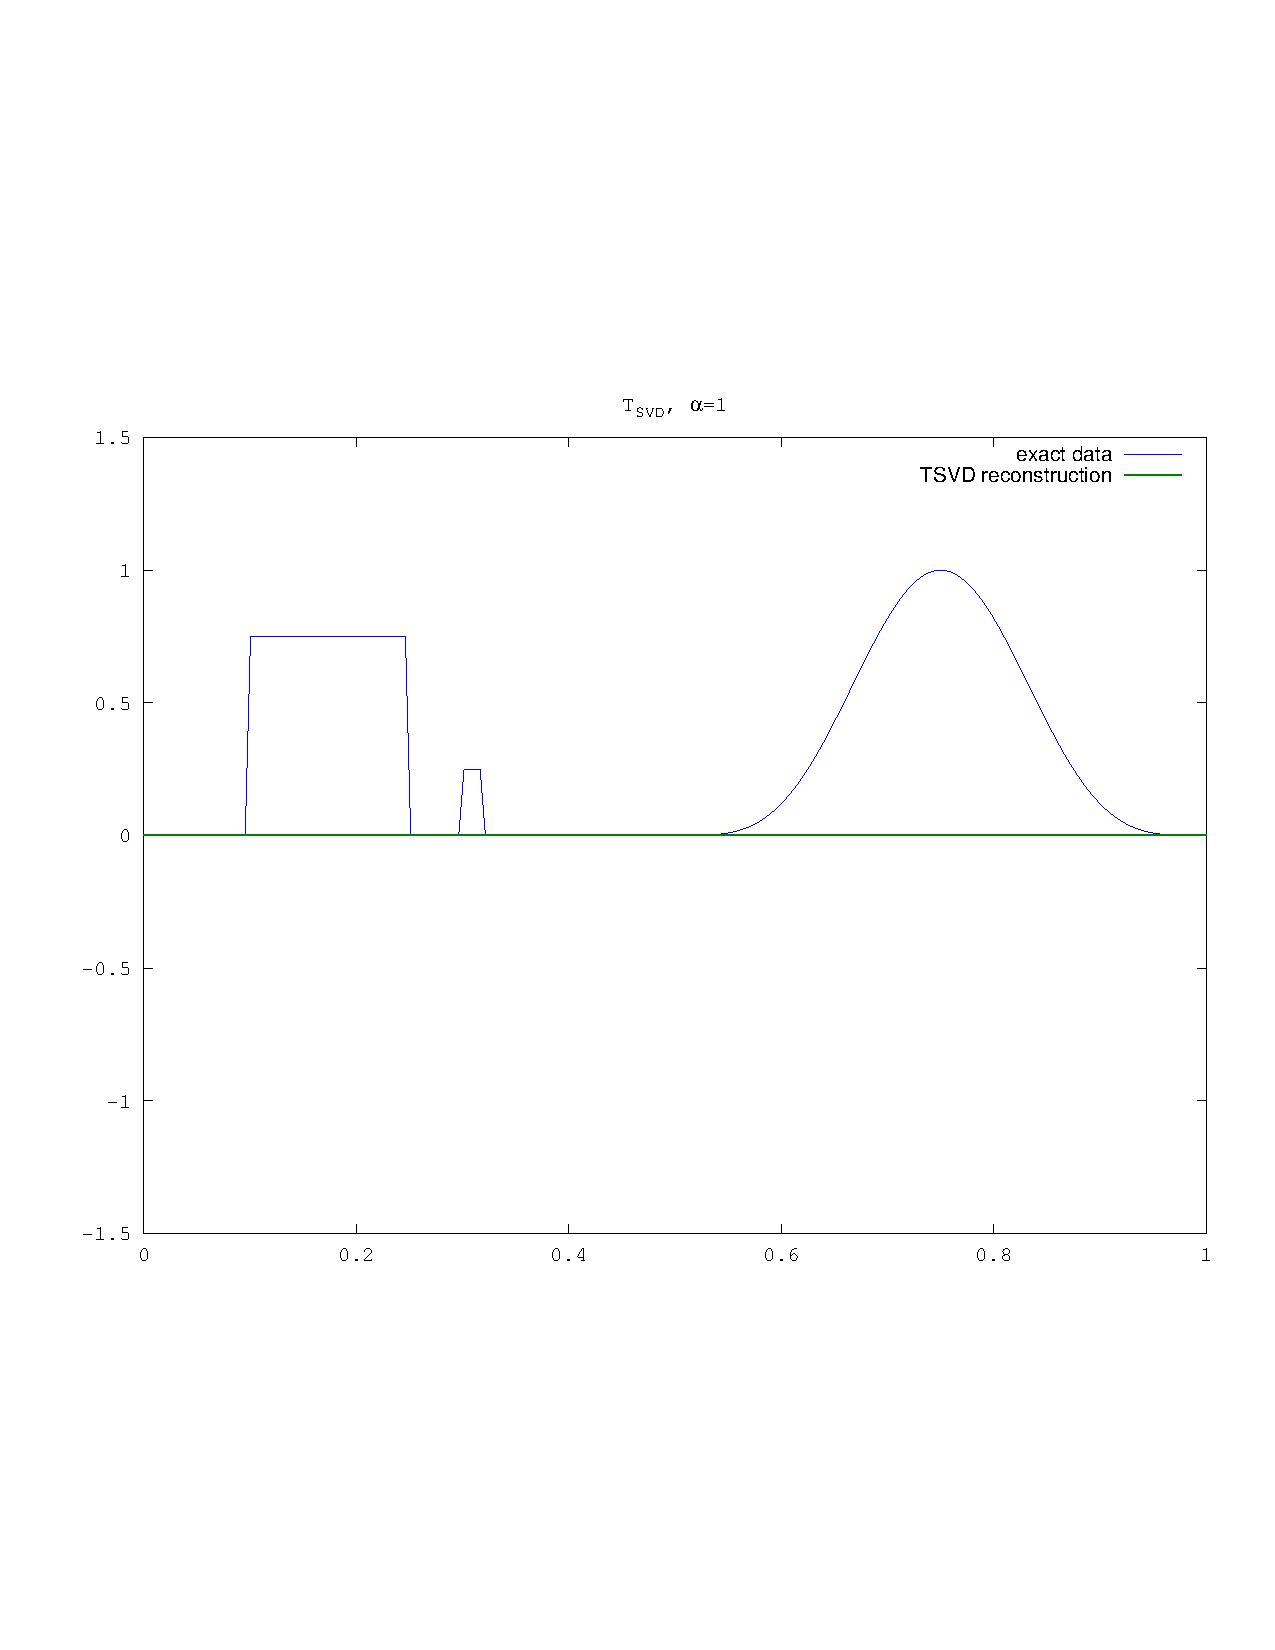
\includegraphics[width=\textwidth]{plots/tsvd1.pdf}
                \caption{$\alpha=1.0$}
        \end{subfigure}
        \caption{$T_{\text{SVD}}$ at varying values of $\alpha$.}
        \label{fig:svd}
\end{figure}

Figure \ref{fig:svd} plots the solution to the inverse problem using
Truncated SVD at several different values of $\alpha$, the
regularization parameter. We can see that actually, the filter nicely
regularizing the inverse problem even for small values of $\alpha$. It
is only for the largest value of $\alpha$ that the parameter is obviously
too large, at which point almost all the frequencies are filtered out,
and the solution to the inverse problem is constant and zero. 

As expected, none of the solutions capture any of the very fine (high
frequency) features of the original data. 

\subsection{L-Curve}

\begin{figure}[!htb]
  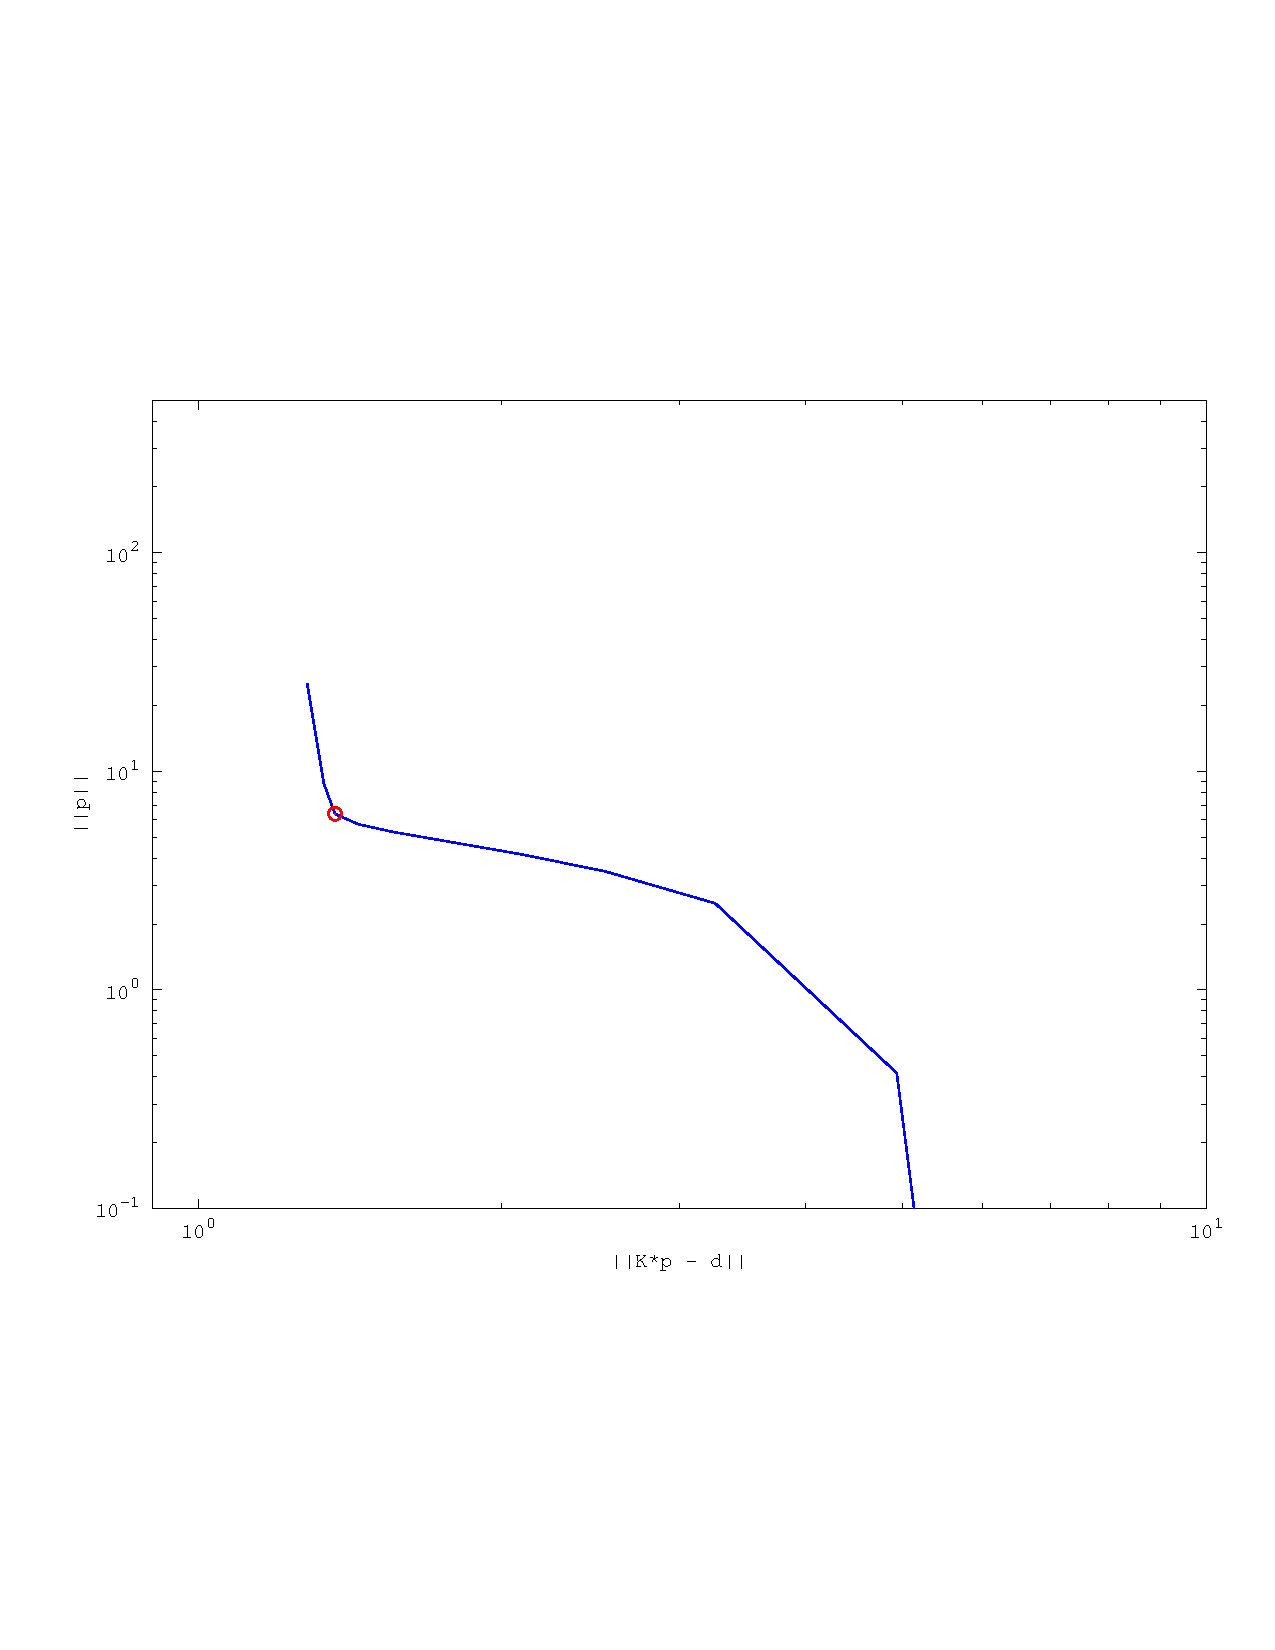
\includegraphics[scale=.6]{plots/L-curve.pdf}
  \caption{The L-curve} 
 \label{fig:lcurve}
\end{figure}

Figure \ref{fig:lcurve} plots the results of the L-curve criterion. The
red dot plotted is at 0.01. This is approximately the ``optimal'' value
of regularization, which is generally consistent with the observations
of the previous plots. 


\end{document}